\documentclass[a4paper]{article}

\usepackage{graphicx}
\usepackage{amsmath}
\usepackage{a4wide}
\usepackage{booktabs}

\title{Identification of the open loop dynamics of a bicycle-rider system under
manual control}
\author{Jason K. Moore and Mont Hubbard}
\date{\today}

\begin{document}

\maketitle

\section{Introduction}

Today's dynamical experiments are capable of delivering a staggering amount of
both kinematic and kinetic data from complex dynamical systems. Such large
amount of data lends itself to data driven modeling approaches that can
potentially provide more predictive models than the traditional building blocks
of dynamical models using first principles. These data driven models can also
give insight into the deficiencies of first principles models. Here we explore
the bicycle-rider system and discuss both traditional models and data driven
models.

The bicycle/motorcycle-rider system has been described with a variety of
models, both simple \cite{Timoshenko1948} and complex \cite{Sharp1971}. Many
studies of bicycles rely on the benchmarked Whipple model \cite{Meijaard2007},
with or without the addition of tire models, for analytical studies of the
system and simulation comparisons. The Whipple bicycle model is regarded as a
highly predictive, yet ``simple'', model of the bicycle-rider system and is
constructed from first principles, yet very little experimental data proves
that the Whipple model is in fact robust at predicting the open loop dynamics
of the bicycle-rider system. The benchmarked Whipple bicycle model
\cite{Meijaard2007} provides a minimalistic standard base model in a manageable
analytic framework capable of describing the essential dynamics such as speed
dependent stability, steer and roll coupling, and non-minimum phase behavior.

We are only aware of two significant experimental attempts at validating the
Whipple model with data generated from bicycle experiments. The most cited,
\cite{Kooijman2008,Kooijman2009}, shows that the Whipple model is predictive of
a \emph{riderless} bicycle in a gymnasium and on a treadmill for speeds in its
predicted stable speed range, 4-6 m/s. \cite{Cain2011} shows that the Whipple
model reduced to a linear steady turn can predict the kinematics, but is not so
good at predicting the rider's input torque.

It is also worth noting that \cite{Eaton1973} and \cite{James2002,James2005}
have identified the open loop dynamics of the motorcycle-rider system. Eaton
used frequency domain identification techniques to identify the dynamics, which
are know to be problematic for closed loop identification \cite{Ljung1999}.
James showed that identified ARX models with lower order than typical first
principles models can predict the measured motion, but does not find very good
agreement with his first principles models.

% TODO : Figure out if Eaton id'd under manual control or not, he may have
% done both

In an attempt to validate the Whipple model, we have collected a large set of
time history data from an instrumented bicycle ridden under manual control. The
measurements include some of the most important kinematic and kinetic variables
describing the bicycle-rider motion from three different riders on the same
bicycle for a variety of maneuvers and speeds. These experiments generated
approximately 1.7 million time samples from each of about 30 sensors sampled at
200 hertz (representing about 2.4 hours of real time).

Our overarching goal was to identify the manual control system employed the
rider, but the schemes we used for control identification relied on an accurate
plant model \cite{Moore2012}. So, we ended up using a solution similar to
\cite{Eaton1973} and identified the plant, i.e. the open loop bicycle and rider
dynamics, first followed by an identification of the control system. We
considered the plant to include the passive, open loop, model of the bicycle
combined with the rider's biomechanics and the controller to be some makeup of
the human brain which takes sensory inputs, has time delays, and sends outputs
for muscular control.

Our preliminary attempts at identifying the controller with the Whipple model
as the system plant showed that the plant always under-predicted the steer
torque needed for a given measured trajectory \cite{Moore2012}. This ultimately
resulted in erroneous estimations of the controller parameters.

As pointed out by many, in particular the motorcycle researchers, there is very
good reason to question some of assumptions in the Whipple model. The main
questionable assumption being knife-edge no side-slip wheels, especially when
under a rider's weight. And secondly, the rider's biomechanics have much more
influence and coupling to the bicycle than the motorcycle, which must be
accounted for.

\section{Instrumented Bicycle}

We developed an instrumented bicycle that had a unique combination of sensors
for dynamic measurements that are known to be important indicators of the
bicycle-rider system motion. The bicycle's primary design criteria were as
follows:

\begin{itemize}
  \item The bicycle should be sized for our intended riders.
  \item The rider's biomechanical movement, including pedaling, should be
    restricted as much as possible so that the Whipple model's rigid rider
    assumption is more probable.
  \item The instrumentation should accurately measure the fundamental
    kinematics of the bicycle: three dimensional rates and orientations of the
    bicycle rear frame, front frame, and wheels.
  \item The instrumentation should accurately measure the rider's applied
    steering torque.
  \item The instrumentation should accurately measure an applied lateral
    disturbance force to the bicycle frame.
  \item The experiments could be performed on open road or on a treadmill.
\end{itemize}

With these criteria in mind we constructed a bicycle with an electric
propulsion system and rigid rider harness and an assortment of sensors. The
rear frame three dimensional angular rates and a three dimensional point
acceleration were measured with a VectorNav VN-100 inertial measurement unit,
the rear frame roll angle was measured with a rotary potentiometer mounted to a
small lightweight trailer, the steer angle was measured with a rotary
potentiometer, the axial torque in the steer tube by a Futek 150 in-lb (±17 Nm)
TFF350 torque sensor, the lateral perturbation force by a load cell 100 lb
force load cell (Interface SSM-100), the angular rate about the steer axis of
the front frame by a rate gyro Single axis rate gyro (Silicon Sensing
CRS03-04S), and the rear wheel angular rate by a DC generator.

\begin{figure}
  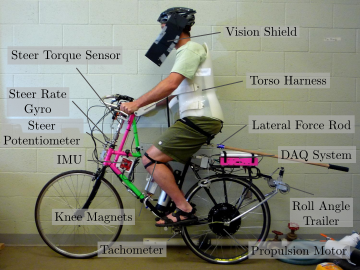
\includegraphics[width=5in]{figures/instrumented-bicycle.pdf}
  \caption{The instrumented bicycle with rider L seated in the harness.}
\end{figure}

\section{Experiments}

The analysis herein focuses on the two maneuvers which we call \emph{Heading
Tracking} and \emph{Lateral Deviation Tracking}. During heading tracking the
rider was instructed to simply balance the bicycle and keep a relatively
constant heading while focusing their vision at a point in the far distance.
During lateral deviation tracking the rider was instructed to focus on a
straight line that was marked on the ground and to attempt to keep the front
wheel on the line.

Both tasks were performed with and without the application of a manually
applied lateral perturbation forces just below the seat. The forces were
applied randomly in direction and time during the trials. Each maneuver was
performed on both a 1 meter wide treadmill and an open gymnasium floor. See
\cite{Moore2012} for the full details.

\section{Data}
\label{sec:data}

The physical parameters (geometry, mass, center of mass, and moments of
inertia) of both the bicycle and the rider were estimated using the methods in
\cite{Moore2012} and \cite{Yeadon1990}. The bicycle was measured to get
accurate estimates of the parameters used in the benchmark model,
\cite{Meijaard2007}. The combined inertial properties of the bicycle rear frame
and the rider were computed with standard methods. Two open source software
packages, \verb|yeadon| \cite{Dembia2011} and \verb|BicycleParameters|
\cite{Moore2011} manage and process the data physical parameter data.

% TODO : add where to get the data

% TODO: Add a table of the whipple model parameters for the three riders

Before each day of testing, base data was collected for the system's sensors
for calibration purposes. Then for each trial a set of meta data and raw time
series were collected from the bicycle's onboard DAQ system. This data was
stored in a HDF5 database for easy querying and retrieval in the data analysis
step. The raw data was then processed to obtain the desired time histories
defined by the Whipple model coordinates:

\begin{table}
  \begin{tabular}{lll}
    Variable                                            & Description                                    & Units \\
    \hline
    $v$                                                 & wheel center speed magnitude                   & m/s \\
    $\delta,\phi,\psi$                                  & steer, roll and yaw angles                     & rad \\
    $\dot{\delta},\dot{\phi},\dot{\psi},\dot{\theta}_B$ & steer, roll, yaw, and rear wheel angular rates & rad/s \\
    $T_\delta,F_{c_l}$                                  & steer torque, lateral perturbation force       & NM, N
  \end{tabular}
\end{table}

The signals were measured and processed as described in \cite{Moore2012}. The
roll and steer accelerations were estimated by numerically differentiating the
roll and steer rate signals. Before identification computations we subtracted
the means over time of the signals that were generally symmetric about zero,
i.e. all but lateral force.  Then all of the signals were filtered with a
second order low pass Butterworth filter at 15 Hz cutoff frequency.

% TODO: example plot of the signals

The experimental data was collected on seven different days and amounted to
about 600 individual trials with three different riders. We used 374 of the
runs for the following analysis.

\section{Identification}
\label{sec:identification}

% TODO : This needs to be reworded to reflect that canoncial id

The linear Whipple model is a 4th order system with roll angle $\phi$, steer
angle $\delta$, roll rate $\dot{\phi}$, and steer rate $\dot{\delta}$ selected
as the independent states and with roll $T_\phi$ and steer $T_\delta$ torques
as the generalized forces and system inputs. In place of the roll torque input,
we extend the model to include a lateral force $F$ acting at a point on the
frame to provide a new input, accurately modelling imposed lateral
perturbations (see \cite{Moore2012} for details).  We also examine a second
candidate model which adds the inertial effects of the rider's arms to the
Whipple model, also described in \cite{Moore2012}. This model was designed to
more accurately account for the fact that the riders were free to move their
arms with the front frame of the bicycle. This model is similar in fashion to
the upright rider in \cite{Schwab2010a}, but with slightly different joint
definitions. Constraints are chosen so that no additional degrees of freedom
are added, keeping the system both tractable and comparable to the benchmarked
Whipple model.

For the identification procedure we make the assumptions that the model is (1)
linear, (2) is fourth order, and (3) we can measure the states and inputs
directly while the system is under closed loop control by the rider. We then
employ the \emph{direct identification} approach to identify the plant.

During all of the experiments there are at least two measured external
(exogenous) inputs: the steer torque and the lateral force. Both inputs are
generated manually, the first from the rider and the second from the person
applying the pulsive perturbation. From the set of measured outputs we selected
the roll and steer angles and rates. The problem can then be formulated as
follows: given the inputs and outputs of the system and some system structure,
what model parameters give the best prediction of the output given the measured
input? This a classic system identification problem.

\subsection{Model structure}

Identification of the bicycle-rider equations of motion can be formulated with
respect to an augmented benchmark canonical form based on \cite{Meijaard2007},
shown in Equation \ref{eq:canonical}. If the time varying quantities in the
equations are all measured at each time step, the coefficients of the linear
equations can be estimated given enough time steps.

\begin{equation}
  \mathbf{M} \ddot{q} + v \mathbf{C}_1 \dot{q} + [g \mathbf{K}_0 + v^2
  \mathbf{K}_2] q = T + H F
  \label{eq:canonical}
\end{equation}

where the time-varying states roll and steer are collected in the vector $q =
[\phi \quad \delta]^T$, the time varying inputs roll torque and steer torque
are collected in the vector $T = [T_\phi \quad T_\delta]^T$, and $H = [H_{\phi
F} \quad H_{\delta F}]^T$ is a vector describing the linear contribution of the
lateral force, $F$, to the roll and steer torque equations. This equation
assumes that the speed, $v$, is constant with respect to time as the model was
linearized about a constant speed equilibrium, but we treat $v$ as a time
varying parameter because the measured longitudinal acceleration is negligible.
The augmented form extends the equations in \cite{Meijaar2007} to properly
account for the lateral perturbation force, $F$, which was the actual input we
delivered during the experiments. The force was applied just below the seat so
most of the contribution from $F$ is in the roll equation.

\subsection{Identification}

A simple analytic identification problem can be formulated from the canonical
form. If we have good measurements of $q$, their first and second derivatives,
forward speed $v$, and the inputs $T_\delta$ and $F$, the entries in
$\mathbf{M}$, $\mathbf{C}_1$, $\mathbf{K}_0$, $\mathbf{K}_2$, and $H$ can be
identified by forming two simple linear regressions (one for each equation
in the canonical form).

The roll and steer equations each can be put into a simple linear form:

\begin{equation}
  \mathbf{\Gamma} \Theta = Y
\end{equation}

where $\Theta$ is a vector of the unknown constant matrix entries and the
design matrix, $\mathbf{\Gamma}$, and the prediction vector, $Y$, are made up
of the inputs and outputs measured during a run. $\Theta$ can be all or a
subset of the entries in the canonical matrices. $\hat{\Theta}$ can be
estimated using the well known linear least squares solution.

\begin{equation}
  \hat{\Theta} = [\mathbf{\Gamma}^T \mathbf{\Gamma}]^{-1} \mathbf{\Gamma}^T Y
  \label{eq:theta-estimate}
\end{equation}

Equation \ref{eq:theta-estimate} can be solved for each run individually, a
portion of a run, or a set of runs.

Also, all of the parameters in the canonical matrices need not be estimated.
The analytical formulation of the Whipple model bicycle model
\cite{Meijaard2007} gives a good idea of which entries in the matrices we may
be more certain about from our physical parameters measurements. We fixed the
parameters if it was a function of trail, front assembly moments and products
of inertia, or equal to zero. This is because the true trail is difficult to
measure, the inertia of the front frame plays a large roll in the steer
dynamics.

For the roll equation this leaves $M_{\phi\delta}$, $C_{1\phi\delta}$,
and $K_{0\phi\delta}$ as free parameters, and for the steer equation
this leaves $M_{\delta\phi}$, $M_{\delta\delta}$, $C_{1\delta\phi}$,
$C_{1\delta\delta}$, $K_{0\delta\phi}$, $K_{0\delta\delta}$,
$K_{2\delta\delta}$, and $H_{\delta F}$ as free parameters.

We start by identifying the three coefficients of the roll equation for
the given data using

\begin{align}
  &\begin{bmatrix}
     \ddot{\delta}(1) &
     v(1) \dot{\delta}(1) &
     g \delta(1) \\
     \vdots & \vdots & \vdots\\
     \ddot{\delta}(N) &
     v(N) \dot{\delta}(N) &
     g \delta(N) \\
  \end{bmatrix}
  \begin{bmatrix}
    M_{\phi\delta} \\
    C_{1\phi\delta} \\
    K_{0\phi\delta}
  \end{bmatrix}\\
  &=
  \begin{bmatrix}
    H_{\phi F} F(1)
    - M_{\phi\phi} \ddot{\phi}(1)
    - C_{1\phi\phi} v(1) \dot{\phi}(1)
    - K_{0\phi\phi} g \phi(1)
    - K_{2\phi\phi} v(1)^2 \phi(1)
    - K_{2\phi\delta} v(1)^2 \delta(1) \\
  \vdots\\
    H_{\phi F} F(N)
    - M_{\phi\phi} \ddot{\phi}(N)
    - C_{N\phi\phi} v(N) \dot{\phi}(N)
    - K_{0\phi\phi} g \phi(N)
    - K_{2\phi\phi} v(N)^2 \phi(N)
    - K_{2\phi\delta} v(N)^2 \delta(N) \\
  \end{bmatrix} \nonumber
\end{align}

We then enforce the assumptions that $M_{\phi\delta} = M_{\delta\phi}$ and
$K_{0\phi\delta} = K_{0\delta\phi}$ to fix these values in the steer equation
to the ones identified in the roll equation, leaving fewer free parameters in
the steer equation. Finally, I identify the remaining steer equation
coefficients with

\begin{align}
  \begin{bmatrix}
    \ddot{\delta}(1) &
    v(1) \dot{\phi}(1) &
    v(1) \dot{\delta}(1) &
    g \phi(1) &
    v(1)^2 \delta(1) &
    - F(1)\\
    \vdots & \vdots & \vdots & \vdots & \vdots & \vdots \\
    \ddot{\delta}(N) &
    v(N) \dot{\phi}(N) &
    v(N) \dot{\delta}(N) &
    g \phi(N) &
    v(N)^2 \delta(N) &
    - F(N)\\
  \end{bmatrix}
  \begin{bmatrix}
    M_{\delta\delta} \\
    C_{1\delta\phi} \\
    C_{1\delta\delta} \\
    K_{0\delta\phi} \\
    K_{2\delta\delta} \\
    H_{\delta F}
  \end{bmatrix} \nonumber \\
  =
  \begin{bmatrix}
    T_\delta(1)
    - M_{\delta\phi} \ddot{\phi}(1)
    - K_{0\delta\delta} g \delta(1)
    - K_{2\delta\phi} v(1)^2 \phi(1) \\
    \vdots\\
    T_\delta(N)
    - M_{\delta\phi} \ddot{\phi}(N)
    - K_{0\delta\delta} g \delta(N)
    - K_{2\delta\phi} v(N)^2 \phi(N) \\
  \end{bmatrix}
\end{align}

\section{Results}

From our larger pool of data, we selected data for three riders on the same
bicycle, performing two maneuvers, in two different environments. There is
little reason to believe the dynamics of the open loop system should vary much
with respect to different maneuvers, but there is potential variation across
riders due to the differences in their inertial and musculoskeletal properties
and there may be variation across environments because of the differences in
the wheel to floor interaction. We computed the best fit model across a series
of runs to benefit from the large dataset. We then selected four scenarios with
a total of 12 different models:

\begin{itemize}
  \item
    All riders in both environments, one data set
  \item
    All riders in each environment, two data sets
  \item
    Each rider in both environments, three data sets
  \item
    Each rider in each environment, six data sets
\end{itemize}

\subsection{Model Quality}

The predictive capability and quality of a given model can be quantified by an
assortment of criteria and methods. We used two criteria to judge the quality
of the identified models with respect to the available data: (1) we compute the
variance accounted for (VAF) (i.e. coefficent of determination) with respect to
the linear least squares solution for each set of run and each identified model
and (2) simulate the identified model given the measured steer torque and
lateral force for each run and compute VAF with respect to the four predicted
outputs and measured outputs.

The second method works well when the open loop system is stable, but if it is
unstable as is so in the case of this bicycle, it may be difficult to simulate.
Searching for initial conditions that give rise to a stable model for the
duration of the run or simulating by weighting the future error less may
relieve the instability issues. We chose the former method for these
computations.

For method (1) the \emph{variance accounted for} (VAF) by the model for both
the roll torque and the steer torque equations are:

\begin{equation}
  \label{eq:vaf}
  \textrm{VAF}_{\phi,\delta} = 1 - \frac{\vert \vert
    \mathbf{\Gamma}_{\phi,\delta}\hat{\Theta}_{\phi,\delta} - Y_{\phi,\delta} \vert \vert}
                            {\vert \vert Y_{\phi,\delta} - \bar{Y}_{\phi,\delta} \vert \vert}
\end{equation}

where $c$ is either $\phi$ or $\delta$ and $\bar{Y}$ is the mean of $Y$.

We compute the two VAF values for each of the subsets of data from the 12
scenario combinations using 13 models: the 12 identified models and the Whipple
model. The columns in tables \ref{tab:roll-r-squared} and
\ref{tab:steer-r-squared} correspond to the models and the rows correspond to
the data subsets the VAF was computed with. The maximum VAF in a row gives an
indication of the best model for predicting that set of runs.

\begin{table}
  \caption{The VAF in the roll equation computed for each subset of data (rows)
  and each model (columns).}
  \label{tab:roll-r-squared}
  \tiny
  \begin{tabular}{lrrrrrrrrrrrrr}
\toprule
{} &   A-A &   A-H &   A-P &   C-A &   C-H &   C-P &   J-A &   J-H &   J-P &   L-A &   L-H &   L-P &  Whipple \\
\midrule
C-H & 29.3\% & 29.6\% & 25.5\% & 30.5\% & 30.9\% & 29.6\% & 28.4\% & 28.2\% & 23.4\% & 27.8\% & 29.8\% & 18.1\% &     5.0\% \\
C-P & 18.3\% & 17.8\% & 17.6\% & 19.1\% & 18.6\% & 19.2\% & 17.6\% & 17.1\% & 16.4\% & 18.0\% & 17.8\% & 14.8\% &     8.7\% \\
C-A & 21.7\% & 21.4\% & 20.1\% & 22.7\% & 22.4\% & 22.5\% & 21.0\% & 20.5\% & 18.7\% & 21.1\% & 21.5\% & 15.9\% &     7.5\% \\
J-H & 30.5\% & 31.1\% & 27.0\% & 28.9\% & 29.5\% & 27.9\% & 30.8\% & 31.2\% & 26.1\% & 29.7\% & 30.3\% & 21.4\% &    -0.4\% \\
J-P & 47.6\% & 44.4\% & 50.0\% & 43.7\% & 43.0\% & 43.7\% & 47.6\% & 44.5\% & 50.5\% & 48.9\% & 41.3\% & 49.4\% &    36.1\% \\
J-A & 35.6\% & 35.1\% & 33.6\% & 33.4\% & 33.6\% & 32.6\% & 35.8\% & 35.3\% & 33.1\% & 35.3\% & 33.7\% & 29.3\% &     9.9\% \\
L-H & 25.5\% & 26.9\% & 20.1\% & 25.9\% & 26.5\% & 24.7\% & 25.1\% & 26.4\% & 18.2\% & 23.8\% & 27.4\% & 12.4\% &    -5.5\% \\
L-P & 47.2\% & 43.5\% & 51.6\% & 43.4\% & 41.8\% & 44.5\% & 47.2\% & 44.3\% & 52.2\% & 49.3\% & 40.2\% & 53.3\% &    48.5\% \\
L-A & 37.8\% & 36.5\% & 37.4\% & 36.0\% & 35.4\% & 36.0\% & 37.6\% & 36.6\% & 36.7\% & 38.1\% & 34.9\% & 34.2\% &    22.7\% \\
A-H & 29.6\% & 30.2\% & 25.7\% & 28.7\% & 29.3\% & 27.7\% & 29.5\% & 30.0\% & 24.4\% & 28.5\% & 29.8\% & 19.5\% &     2.8\% \\
A-P & 34.9\% & 33.0\% & 36.2\% & 33.4\% & 32.6\% & 33.7\% & 34.6\% & 32.8\% & 36.0\% & 35.7\% & 31.3\% & 35.0\% &    27.4\% \\
A-A & 32.1\% & 31.5\% & 30.5\% & 30.9\% & 30.8\% & 30.4\% & 31.9\% & 31.3\% & 29.6\% & 31.8\% & 30.5\% & 26.4\% &    13.6\% \\
\bottomrule
\end{tabular}

\end{table}

\begin{table}
  \caption{The VAF in the steer equation computed for each subset of data (rows)
  and each model (columns).}
  \label{tab:steer-r-squared}
  \tiny
  \begin{tabular}{lrrrrrrrrrrrrr}
\toprule
{} &  A-A &  A-H &  A-P &  C-A &  C-H &  C-P &  J-A &  J-H &  J-P &  L-A &  L-H &  L-P &  Whipple \\
\midrule
A-A & 66.8 & 66.9 & 61.3 & 62.7 & 64.9 & 50.6 & 66.8 & 64.5 & 66.3 & 62.4 & 62.7 & 56.4 &     65.5 \\
A-H & 68.0 & 68.4 & 60.2 & 63.4 & 67.9 & 47.4 & 67.5 & 65.4 & 66.2 & 63.2 & 64.8 & 55.2 &     66.8 \\
A-P & 64.8 & 64.4 & 63.5 & 61.4 & 60.0 & 56.9 & 65.6 & 63.0 & 66.4 & 60.9 & 59.3 & 58.6 &     63.1 \\
C-A & 52.9 & 55.3 & 47.1 & 48.4 & 51.9 & 39.1 & 56.0 & 54.9 & 52.6 & 45.8 & 47.7 & 40.2 &     56.7 \\
C-H & 58.3 & 60.8 & 49.4 & 53.1 & 59.1 & 38.4 & 60.8 & 59.0 & 56.8 & 50.6 & 53.5 & 42.3 &     61.4 \\
C-P & 48.5 & 50.7 & 45.0 & 44.4 & 46.1 & 39.8 & 52.0 & 51.3 & 49.0 & 41.8 & 42.9 & 38.3 &     52.7 \\
J-A & 70.7 & 70.0 & 65.0 & 66.8 & 68.8 & 53.8 & 69.4 & 67.0 & 69.6 & 67.4 & 67.8 & 60.7 &     68.5 \\
J-H & 70.2 & 69.9 & 62.9 & 66.0 & 70.0 & 50.2 & 68.9 & 66.8 & 68.2 & 66.2 & 67.5 & 58.5 &     68.7 \\
J-P & 72.3 & 70.3 & 71.6 & 69.2 & 65.6 & 65.4 & 71.0 & 67.6 & 73.5 & 70.7 & 68.5 & 67.8 &     68.1 \\
L-A & 70.1 & 69.5 & 65.3 & 65.2 & 66.8 & 52.1 & 70.0 & 66.7 & 71.2 & 65.4 & 63.7 & 60.4 &     67.7 \\
L-H & 67.8 & 68.5 & 58.7 & 61.9 & 67.2 & 43.6 & 67.6 & 65.2 & 66.4 & 62.3 & 63.7 & 53.6 &     67.0 \\
L-P & 72.6 & 70.6 & 73.7 & 68.9 & 66.5 & 62.9 & 72.7 & 68.3 & 77.3 & 68.9 & 63.7 & 69.1 &     68.6 \\
\bottomrule
\end{tabular}

\end{table}

\begin{itemize}
  \item
    The arm model is poor at predicting the steer torque.
  \item
    The models derived from rider C's runs are poorer at predicting the inputs.
  \item
    The Whipple model is not too bad at predicting steer torque, but on
    average about 10\% worse than the best models.
  \item
    The models identified from the pavilion runs are generally the best (with
    exception of C's). The ones generated from L and J's runs are typically the
    best at predicting both steer torque and roll torque, with L's giving
    better roll torque predictions.
  \item
    The roll torque is poorly predicted by all models when it is supposed
    to be zero. This raises implications in the validity of the roll
    equation and the potential need for tire slip models.
\end{itemize}

For method (2), we simulate all 14 models with the inputs measured from the 374
runs and compute the VAF explained by the model for each of the four outputs.
Since the models are typically unstable at all of the speeds we tested, we
searched for the set of initial conditions which minimizes the VAF for all
outputs and ignored any runs in which suitable initial confiditions couldn't be
found. Table \ref{tab:MedianVAFOutputs} presents the median percent variance
accounted for across all runs for the outputs of each model. Based on the mean
VAF across the outputs for each model the best model seems to be L-P. Notice
that the Whipple model is the poorest predictor and the arm model is the second
poorest.

% TODO : It'd be nice to know the number of runs used in each median
% computation.
\begin{table}
  \label{tab:MedianVAFOutputs}
  \caption{The median VAF of each output variable over 374 runs for each model
  and the mean of the median VAFs.}
  \centering
  \begin{tabular}{lrrrrr}
            & $\phi$   & $\delta$ & $\dot{\phi}$ & $\dot{\delta}$ & Mean   \\
    \hline
    A-A     & 28.6\%   & 61.8\%   & 51.8\%      & 65.2\%          & 51.8\% \\
    C-H     & 18.6\%   & 57.2\%   & 52.6\%      & 62.2\%          & 47.7\% \\
    L-A     & 29.4\%   & 59.8\%   & 52.9\%      & 67.9\%          & 52.5\% \\
    A-H     & 24.1\%   & 57.4\%   & 43.1\%      & 64.2\%          & 47.2\% \\
    C-A     & 14.9\%   & 54.5\%   & 51.7\%      & 59.8\%          & 45.2\% \\
    J-P     & -3.4\%   & 35.4\%   & 34.1\%      & 61.7\%          & 31.9\% \\
    L-H     & 24.3\%   & 57.7\%   & 46.1\%      & 65.7\%          & 48.5\% \\
    A-P     & 29.7\%   & 58.9\%   & 60.6\%      & 63.2\%          & 53.1\% \\
    J-H     & 22.8\%   & 53.6\%   & 42.0\%      & 62.8\%          & 45.3\% \\
    L-P     & 38.2\%   & 62.8\%   & 60.9\%      & 68.4\%          & 57.6\% \\
    C-P     & 19.0\%   & 46.0\%   & 42.0\%      & 47.1\%          & 38.5\% \\
    J-A     & 27.9\%   & 61.0\%   & 49.4\%      & 65.9\%          & 51.1\% \\
    Whipple & -21.0\%  & 10.3\%   & 5.8\%       & 12.2\%          &  1.8\% \\
    Arm     & -33.1\%  & 19.6\%   & 29.7\%      & 33.1\%          & 12.3\% \\
  \end{tabular}
\end{table}

\begin{itemize}
  \item
    For all outputs other than roll angle, the arm model is better than
    the Whipple model.
  \item
    The models from C's data fare much better than the input comparisons and
    are better than some of J's.
  \item
    The model identified from the data with rider J on the Pavilion floor is
    very poor in roll angle prediction as opposed to being a good choice from
    the input comparison results.
  \item
    All of the identified models are better predictors than the first
    principles models.
\end{itemize}

\subsection{Most predicitive model}
% TODO : show results of the L-P model here instead.

This section details the characterisitcs for the identified model which best
predicts \emph{all} of the data, the L-P model.

The eigenvalues as a function of speed of the identified model can be compared
to those of the Whipple and arm models. Figure \ref{fig:AARloc} shows the root
locus of the three models as a function of speed. The oscillatory weave mode
exists in all three models, stable at all speeds in the arm model but unstable
at lower speeds in the other two models. The identified model's oscillatory
weave mode is unstable over most of the shown speed range. Above 3 m/s or so,
the Whipple model's oscillatory weave mode diverges from the identified model
to different asymptotes. The arm model weave mode diverges somewhere in
between. Note that the arm model has an unstable real mode for all speeds.

Figure \ref{fig:AAEig} gives a different view of the root locus allowing one to
more easily compare the real and imagrinary parts of the eigenvalues
indenpendently. The imaginary parts of the weave mode have similar curvature
with respect to speed for all the models, with the identified model having
about 1 rad/s larger frequency of oscillation for all speeds. The identified
model does have a stable speed range where the Whipple model under predicts the
weave critical speed by almost 2 m/s. The identified caster mode is much faster
than the one predicted by the Whipple model which is somewhat counterintuitive
because tire scrub torques would probably tend to slow the caster mode.
Although, the pneumatic trail and the rider's arm inertia could play a larger
role that expected. Furthermore, the caster mode may not be well identified
because the experiments were not design to specifically excite it.

\begin{figure}
  \includegraphics[width=5in]{figures/L-P-rlocus.pdf}
  \caption{Root locus of the identified model (circle), the Whipple model
    (diamond), and the arm model (triangle) with respect to speed in m/s.
    }
\end{figure}

\begin{figure}
  \includegraphics[width=5in]{figures/L-P-eig.pdf}
  \caption{Real and imaginary parts of the eigenvalues as a function of speed
    for model (I)dentified from all runs, the (W)hipple model and the (A)rm
  model.}
\end{figure}

The frequency band from 1 rad/s to 12 rad/s is of most concern as it bounds a
reasonable range that the human may be able to operate within. The steer torque
to roll angle transfer function, Figure
11.15\textless{}figAATdelPhi\textgreater{} may be the most important to model
accurately as it is the primary method of controlling the bicycle's direction,
i.e. commanding roll allows one to command yaw. At 2 m/s the Whipple model
magnitude matches at lower frequencies (\textless{} 4 rad/s) better and the arm
model better at higher frequencies (\textgreater{} 4 rad/s). A 4 m/s and above
the magnitude of identified varies little with speed, which contrasts the
stronger speed dependence of the first principles models. The low frequency
behavior of the identified model is not well predicted by the Whipple and arm
models at the three highest speeds but about about 3 rad/s the arm model shows
better magnitude matches than the Whipple model.

\begin{figure}
  \includegraphics[width=5in]{figures/L-P-Tdel-Phi.pdf}
  \caption{Frequency response of the three models, (I)dentified, (W)hipple, and
    (A)rm, at four speeds (2, 4, 6, and 9 m/s). The color indicates the model
    and the line type indicates the speed}
\end{figure}

% TODO : The H values are the same, somethings fishy.
\begin{table}
  \begin{tabular}{lccccc}
  Model & $\mathbf{M}$ & $\mathbf{C}_1$ & $\mathbf{K}_0$ & $\mathbf{K}_2$ & $H$ \\
  \hline \\[0.0625in]
  Whipple &
  $\begin{bmatrix}
    129.362 & 2.260 \\
    2.260 & 0.219 \\
  \end{bmatrix}$
  &
  $\begin{bmatrix}
    0.000 & 41.622 \\
    -0.315 & 1.376 \\
  \end{bmatrix}$
  &
  $\begin{bmatrix}
    -115.707 & -2.361 \\
    -2.361 & -0.737 \\
  \end{bmatrix}$
  &
  $\begin{bmatrix}
    0.000 & 103.943 \\
    0.000 & 2.190 \\
  \end{bmatrix}$
  &
  $\begin{bmatrix}
    0.902 \\
    0.011 \\
  \end{bmatrix}$ \\[0.125in]
  L-P &
  $\begin{bmatrix}
    129.362 & 2.559 \\
    2.559 & 0.250 \\
  \end{bmatrix}$
  &
  $\begin{bmatrix}
    0.000 & 33.526 \\
    -0.549 & 2.100 \\
  \end{bmatrix}$
  &
  $\begin{bmatrix}
    -115.707 & -4.526 \\
    -4.526 & -0.489 \\
  \end{bmatrix}$
  &
  $\begin{bmatrix}
    0.000 & 103.943 \\
    0.000 & 2.603 \\
  \end{bmatrix}$
  &
  $\begin{bmatrix}
    0.902 \\
    0.011 \\
  \end{bmatrix}$
\end{tabular}
\end{table}

\section{Discussion}

We have shown that a fourth order linear model is adequate for describing the
motion of the bicycle under manual control in a speed range from approximately
1.5 m/s to 9 m/s. Results from this study show that higher order models may
not be necessary for predicting the bicycle-rider plant dynamics. This is an
important finding, as many researchers develop models using first principles
which have orders much greater than 4, with degrees of freedom associated with
tire slip, frame flexibilities, and rider biomechanics, which may be overkill
for many prediction purposes. But, results also reveal that fourth order
archetypal first principles models are not predictive enough to fully describe
the dynamics. These deficiencies are most likely due to un-modeled effects,
with knife-edge, no side-slip wheel contact assumptions being the most probable
candidate. Un-modeled rider biomechanics such as passive arm stiffness and
damping and head motion may play a role too. It is likely that something as
simple as a ``static'' tire scrub torque is needed to improve the fidelity of
the Whipple first principles derivations, but that doesn't preclude that the
addition of a tire slip model, adding more degrees of freedom, might also
improve the predictive ability.

\section*{Acknowledgements}

This paper is based on work supported by the National Science Foundation under
Grant No 0928339. Karl {\AA}str{\"o}m gave me the ideas for the canonical form.

%\printbibliography

\bibliographystyle{plain}
\bibliography{references}

\end{document}
